%% -*- coding: utf-8 -*-
\documentclass[12pt,a4paper]{scrartcl} 
\usepackage[utf8]{inputenc}
\usepackage[english,russian]{babel}
\usepackage{indentfirst}
\usepackage{misccorr}
\usepackage{graphicx}
\usepackage{amsmath}
\usepackage{listings}
\usepackage{xcolor}
\usepackage{float}
\lstset{
  language=JavaScript,
  basicstyle=\ttfamily\small,
  keywordstyle=\color{blue},
  commentstyle=\color{gray},
  stringstyle=\color{green},
  numberstyle=\tiny\color{gray},
  stepnumber=1,
  numbersep=10pt,
  backgroundcolor=\color{white},
  showspaces=false,
  showstringspaces=false,
  showtabs=false,
  frame=none, 
  tabsize=2,
  captionpos=b,
  breaklines=true,
  breakatwhitespace=false,
  title=\lstname
}
\begin{document}
	\begin{titlepage}
		\begin{center}
			\large
			МИНИСТЕРСТВО НАУКИ И ВЫСШЕГО ОБРАЗОВАНИЯ РОССИЙСКОЙ ФЕДЕРАЦИИ
			
			Федеральное государственное бюджетное образовательное учреждение высшего образования
			
			\textbf{АДЫГЕЙСКИЙ ГОСУДАРСТВЕННЫЙ УНИВЕРСИТЕТ}
			\vspace{0.25cm}
			
			Инженерно-физический факультет
			
			Кафедра автоматизированных систем обработки информации и управления
			\vfill

			\vfill
			
			\textsc{Отчет по практике}\\[5mm]
			
			{\LARGE Программаная реализация численного метода \textit{Решение системы линейных алгебраических уравнений методом Гаусса-Жордана}}
			\bigskip
			
			1 курс, группа 1ИВТ АСОИУ
		\end{center}
		\vfill
		
		\newlength{\ML}
		\settowidth{\ML}{«\underline{\hspace{0.7cm}}» \underline{\hspace{2cm}}}
		\hfill\begin{minipage}{0.5\textwidth}
			Выполнил:\\
			\underline{\hspace{\ML}} Д.\,А.~Шалаев\\
			«\underline{\hspace{0.7cm}}» \underline{\hspace{2cm}} 2024 г.
		\end{minipage}%
		\bigskip
		
		\hfill\begin{minipage}{0.5\textwidth}
			Руководитель:\\
			\underline{\hspace{\ML}} С.\,В.~Теплоухов\\
			«\underline{\hspace{0.7cm}}» \underline{\hspace{2cm}} 2024 г.
		\end{minipage}%
		\vfill
		
		\begin{center}
			Майкоп, 2024 г.
		\end{center}
	\end{titlepage}

    % Основное содержание документа
    \newpage
    
    % Введение
\section{Введение}
    \label{sec:intro}
    \subsection{Текстовая формулировка задачи (Вариант 2)}
	Написать программу для решения системы линейных алгебраических уравнений методом Гаусса-Жордана.
    \subsection{Теория метода}

    Метод Гаусса — Жордана (метод полного исключения неизвестных) — метод, который используется для решения квадратных систем линейных алгебраических уравнений, нахождения обратной матрицы, нахождения координат вектора в заданном базисе или отыскания ранга матрицы. Метод является модификацией метода Гаусса. 
	
\textbf{Алгоритм}	
    \begin{enumerate}
        \item Выбирают первый слева столбец матрицы, в котором есть хоть одно отличное от нуля значение.
        \item Если самое верхнее число в этом столбце ноль, то меняют всю первую строку матрицы с другой строкой матрицы, где в этой колонке нет нуля.
        \item Все элементы первой строки делят на верхний элемент выбранного столбца.
        \item Из оставшихся строк вычитают первую строку, умноженную на первый элемент соответствующей строки, с целью получить первым элементом каждой строки (кроме первой) ноль.
        \item Далее проводят такую же процедуру с матрицей, получающейся из исходной матрицы после вычёркивания первой строки и первого столбца.
        \item После повторения этой процедуры \(n-1\) раз получают верхнюю треугольную матрицу.
        \item Вычитают из предпоследней строки последнюю строку, умноженную на соответствующий коэффициент, с тем, чтобы в предпоследней строке осталась только 1 на главной диагонали.
        \item Повторяют предыдущий шаг для последующих строк. В итоге получают единичную матрицу и решение на месте свободного вектора (с ним необходимо проводить все те же преобразования).
    \end{enumerate}
\section{Ход работы}
    \subsection{Выбор средств для разработки}
    Для создания программы, решающей систему линейных алгебраических уравнений методом Гаусса — Жордана, я выбрал язык программирования TypeScript и фреймворк Angular 17 для разработки веб-приложений. Такой выбор был сделан для того, что бы обеспечить использование программы не только на ПК, но и на мобильных устройствах.
    \subsection{Код приложения} 
\begin{lstlisting}[language=JavaScript, caption=Gauss-Jordan Elimination Function]
gaussJordanElimination(matrix: number[][]): { solution: number[], reducedMatrix: number[][] } {
  let n = matrix.length;
  let m = matrix[0].length - 1;
  let reducedMatrix = matrix.map(row => row.slice());
  for (let i = 0; i < n; i++) {
    let maxEl = Math.abs(reducedMatrix[i][i]);
    let maxRow = i;
    for (let k = i + 1; k < n; k++) {
      if (Math.abs(reducedMatrix[k][i]) > maxEl) {
        maxEl = Math.abs(reducedMatrix[k][i]);
        maxRow = k;
      }
    }
    for (let k = i; k < m + 1; k++) {
      let tmp = reducedMatrix[maxRow][k];
      reducedMatrix[maxRow][k] = reducedMatrix[i][k];
      reducedMatrix[i][k] = tmp;
    }
    if (reducedMatrix[i][i] !== 0) {
      for (let k = i + 1; k < m + 1; k++) {
        reducedMatrix[i][k] /= reducedMatrix[i][i];
      }
      reducedMatrix[i][i] = 1;
    } else {
      continue;
    }
    for (let k = 0; k < n; k++) {
      if (k != i) {
        let c = reducedMatrix[k][i];
        for (let j = i; j < m + 1; j++) {
          reducedMatrix[k][j] -= c * reducedMatrix[i][j];
        }
        reducedMatrix[k][i] = 0;
      }
    }
  }
  let solution = new Array(n);
  for (let i = 0; i < n; i++) {
    solution[i] = parseFloat(reducedMatrix[i][m].toFixed(10));
  }
  return { solution, reducedMatrix };
}
\end{lstlisting}

\section{Скриншоты программы}
\label{sec:program-shots}
Пример внешнего вида программы представлен на рис. 1 и рис. 2.
\begin{figure}[H]
    \centering
    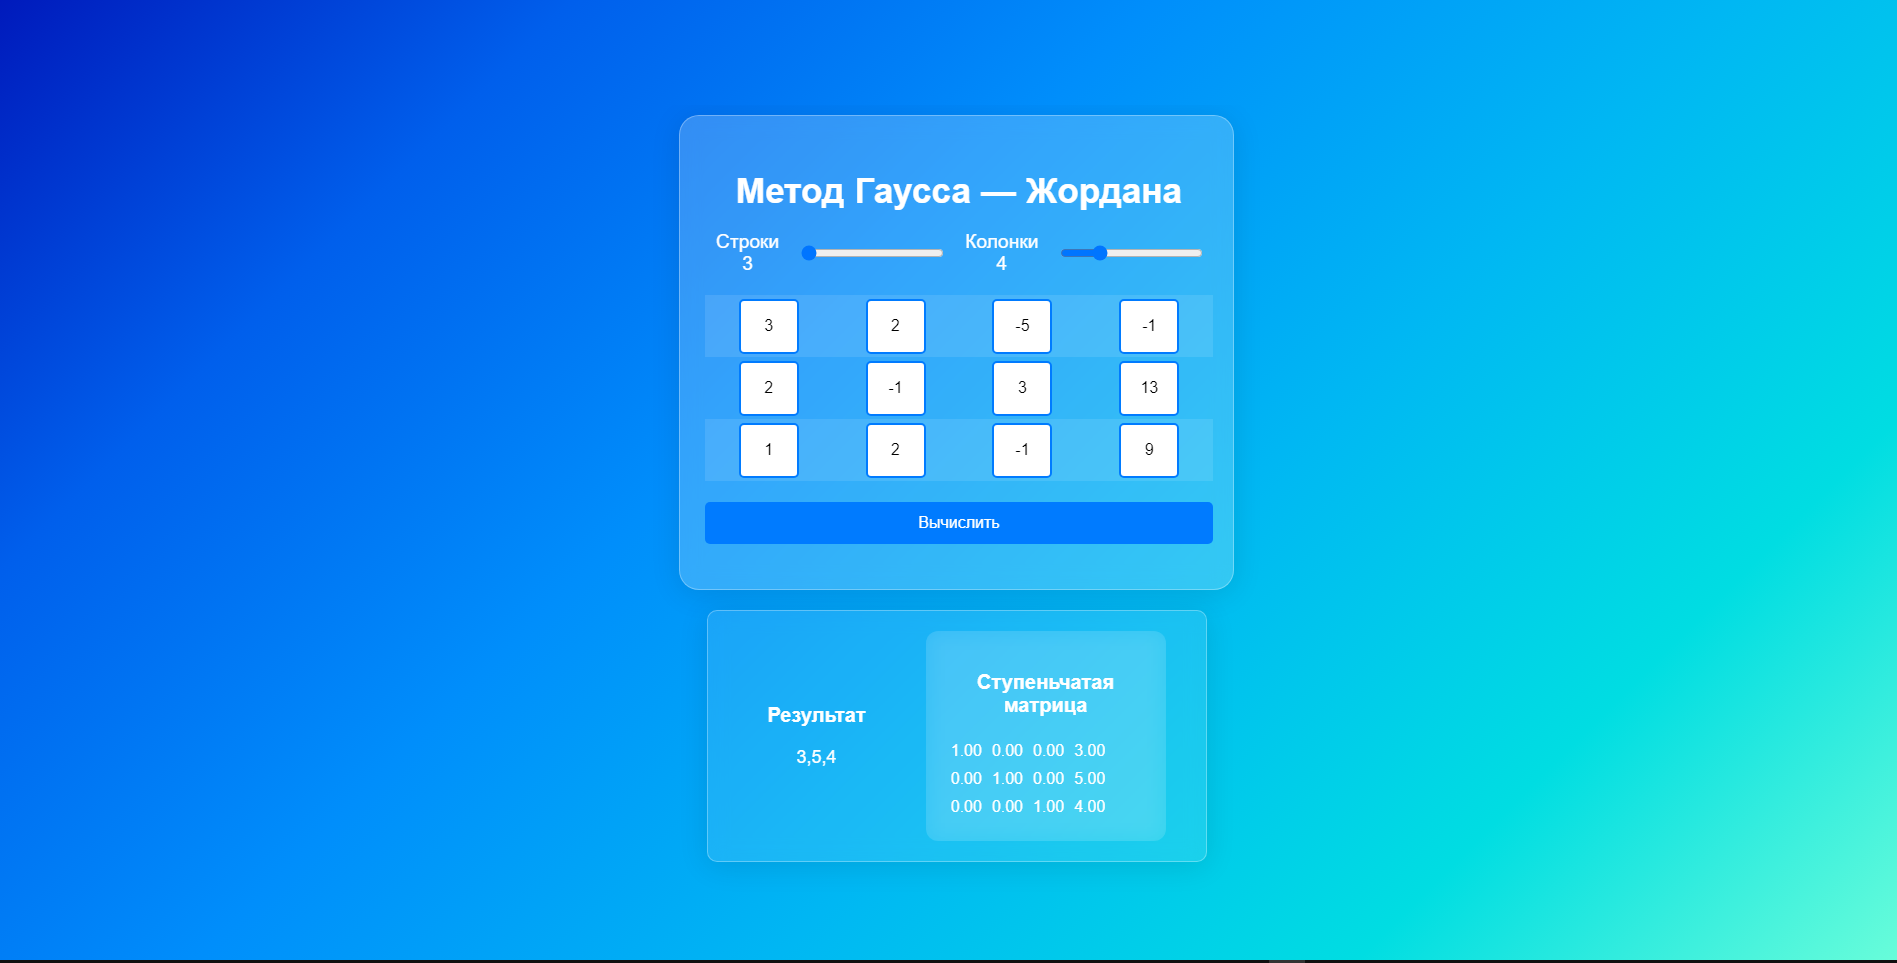
\includegraphics[width=1\linewidth]{PCVersion.png}
    \caption{Внешний вид программы на ПК}
    \label{fig:enter-label}
\end{figure}
\begin{figure}[H]
    \centering
    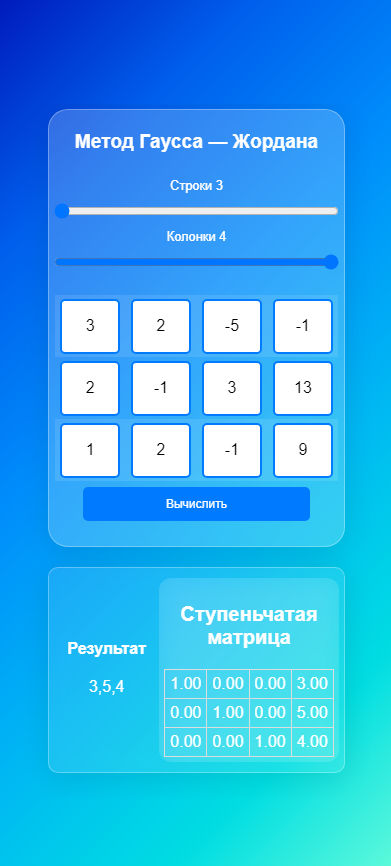
\includegraphics[width=0.25\linewidth]{PhoneVersion.png}
    \caption{Внешний вид программы на мобильных устройствах}
    \label{fig:enter-label}
\end{figure}

    \section{Источники}
    
\begin{thebibliography}{9}
\bibitem{Knuth-2003}Кнут Д.Э. Всё про \TeX. \newblock --- Москва: Изд. Вильямс, 2003 г. 550~с.
\bibitem{Lvovsky-2003}Львовский С.М. Набор и верстка в системе \LaTeX{}. \newblock --- 3-е издание, исправленное и дополненное, 2003 г.
\bibitem{Voroncov-2005}Воронцов К.В. \LaTeX{} в примерах. 2005 г.
\bibitem{Angular17docs-2024}Документация Angular 17. \newblock --- https://v17.angular.io/docs, 2024 г.
\bibitem{TypeScriptdocs-2024}Документация TypeScript. \newblock --- https://www.typescriptlang.org/docs, 2024 г.
\bibitem{TypeScriptcheatsheets-2024}TypeScript CheatSheets. \newblock --- https://www.typescriptlang.org/cheatsheets, 2024 г.
    \end{thebibliography}
\end{document}